%% This is an example first chapter.  You should put chapter/appendix that you
%% write into a separate file, and add a line \include{yourfilename} to
%% main.tex, where `yourfilename.tex' is the name of the chapter/appendix file.
%% You can process specific files by typing their names in at the 
%% \files=
%% prompt when you run the file main.tex through LaTeX.
\chapter{Discrete Element Method}
As described generally in Chapter 1, the discrete element method (DEM) models a system of grains by modeling each grain as a separate entity and calculates the dynamics of each grain by integrating what essentially amounts to $\Sigma\bold{f}=m\bold{a}$ through time. In 2D, each grain is modeled as a disk with a radius $r$, parameterized by three degrees of freedom: two for the center of mass position of the disk (held by a position vector $\bold{x_d}\subset\mathbb{R}^2$), and a third for the rotation of the disk relative to some rest state. The dynamics are captured by another three parameters: two for the center of mass velocity and a third for the angular velocity about the center of mass. In 3D this representation is generalized to a sphere, again with radius $r$ and six degrees of freedom: three for the center of mass ($\bold{x_d}\subset\mathbb{R}^3$) position and three for the angles that describe grain orientation. The dynamics analogously generalize to six parameters, with three for center of mass velocity and three for angular velocities. For a system of $K$ particles, the degrees of freedom of all particles can be concatenated into a single degree of freedom list, the generalized coordinate vector $\bold{q_d}$. In 2D, $\bold{q_d}\subset\mathbb{R}^{3K}$ and in 3D, $\bold{q_d}\subset\mathbb{R}^{6K}$. A generalized velocity vector, $v_d$ can be similarly defined, with $\bold{v_d}\subset\mathbb{R}^{3K}$ in 2D and $ \bold{v_d}\subset\mathbb{R}^{6K}$ in 3D. Momentum balance for the whole granular system can then be summarized with
$$M_d\bold{a_d}=\bold{f_d}(\bold{q_d},\bold{v_d},t)$$
where $M_d\subset\mathbb{R}^{3Kx3K}$ (2D) and $M_d\subset\mathbb{R}^{6Kx6K}$ (3D) is the mass matrix, $\bold{a_d}\subset\mathbb{R}^{3K}$ (2D) and $\bold{a_d}\subset\mathbb{R}^{6K}$ (3D) is the generalized acceleration vector, and $\bold{f_d}$ is the force vector that encapsulates all internal and external forces of the system. The evolution of the system configuration can then be described with 
$$\bold{\dot{q_d}}=\hat{\dot{\bold{q_d}}}(\bold{q_d},\bold{v_d},\bold{a_d})$$
where $\hat{\dot{\bold{q_d}}}$ is a function that encapsulates configuration updates.

\subsection{DEM Model} \label{DEM_Model}
The construction of $\bold{f_d}$, and specifically the contact model that goes into $\bold{f_d}$, has been the source of much work. Popular contact models include Hertzian contact and linear spring-dashpot systems, the latter of which we use \textcolor{red}{FINDREFERENCE}. While Hertzian contact in theory accounts for a nonlinear penalty force with respect to penetration depth due to geometric considerations not present in the simple Hookean spring model, the simplicity of the Hookean spring model along with its acceptable accuracy from literature motivate the latter's use in the current study \textcolor{red}{FINDREFERENCE}. 

\begin{figure}[htp] 
    \centering
    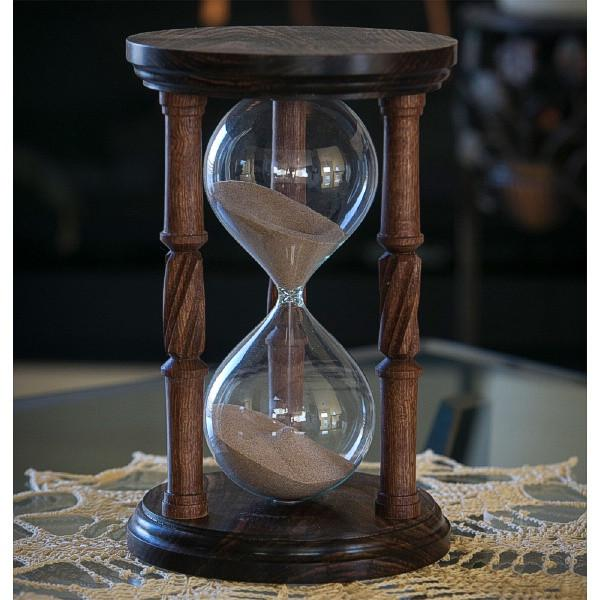
\includegraphics[width=0.4\textwidth]{figs/hourglass_whole.jpg}
    \caption{Two disks in contact with relevant properties labeled for DEM.}
    \label{DEM_diagram}
\end{figure}

In the current work, the contact force, $\bold{f_c}$, is a linear combination of a normal contact force $\bold{f_n}$ and tangential contact force $\bold{f_t}$, such that simply $\bold{f_c} = \bold{f_n} + \mu\bold{f_t}$, where $\mu$ is the coefficient of friction. $\bold{f_d}$ more concretely is
$$\bold{f_n}=k_nd\bold{n}-\gamma_n\bold{v_n}$$
where $k_n$ is the Hookean spring constant in the normal direction, $d$ is the penetration depth between the two disks, $\bold{n}$ is the contact normal unit vector, $\gamma_n$ is the normal damping coefficient, and $\bold{v_n}$ is the normal component of the relative velocity between the two disks. Similarly, the tangential contact force is given by
$$\bold{f_nt}=k_t\Delta\bold{s}-\gamma_t\bold{v_t}$$
where $k_t$ is the spring constant in the tangential direction, $\gamma_t$ is the tangential damping coefficient, and $\bold{v_t}$ is the tangential component of the relative velocity. Friction is captured in this model by requiring that
$$\bold{f_t}\leq\mu\bold{f_n}$$
which is accomplished by adjusting $\Delta\bold{s}$. For a given enduring contact over time, $\Delta\bold{s}$ for that contact is the time integral of the tangential relative velocity during that contact. $\Delta\bold{s}$ is then rescaled so that it $\bold{f_t}$ falls within the friction cone determined by $\mu\bold{f_n}$.

With the given spring-dashpot system, a coefficient of restitution (COR) $e$ can be tuned as a function of the model parameters. Given a desired $e$ and a normal spring coefficient $k_n$, $\gamma_n$ is determined as
$$\gamma_n=\sqrt{mk_n}(-2\log{e})/\sqrt{2(\pi^2+\log{e}^2}$$
where $m$ is the mean mass of a grain \cite{Kamrin:2014}. Note that the use of a "mean" mass is due to the fact that in all of the simulations conducted in this study, a slight polydispersity in granular radii is used with a single density for all particles, resulting in a mass distribution. This is done to better match real shape distributions in a granular system, and to avoid crystallization that commonly arises in monodisperse systems. The choice of $k_n$ and other material parameters is further explained for specific simulations later in the study, but in general is chosen to be as stiff as possible while still retaining a reasonable cost per time step, with a timestep usually on the order of $10^{-6}$ seconds.

\subsection{DEM Algorithm}
The DEM code used in this study was built completely in house, though is similar in general algorithmic structure to many DEM codes that exist, such as LAMMPS or LIGHTS \textcolor{red}{FINDREFERENCE}. Thus for transparency as well as necessity when later explaining the hybrid algorithm, the structure of the used DEM code is discussed.

\begin{algorithm}
  \caption{${\tt Overall \_ DEM \_ Algorithm}$}
  \begin{algorithmic}[1]
  \State ${\tt Broad\_Phase\_Collision\_Detection}$
  \For{$i=0 \dots num\_possible\_collisions$}
    \State ${\tt Narrow\_Phase\_Collision\_Detection}$
  \EndFor
  \State ${\tt Collision\_Update}$
  \For{$each\_collision\_type$}
    \State ${\tt Update\_Properties}$
    \State ${\tt Integrate\_\Delta\bold{s}}$
  \EndFor
  \State ${\tt Force\_Update}$ 
  \For{$each\_collision$}
    \State ${\tt Calculate\_Penalty\_Force}$
    \State ${\tt Correct\_\Delta\bold{s}}$
    \State ${\tt Add\_Force\_To\_Contact\_Grains}$
  \EndFor
  \State ${\tt Time\_Integration}$ 
  \end{algorithmic}
  \label{alg:DEM_algorithm}
\end{algorithm}

The $Broad\_Phase\_Collision\_Detection$ creates an axis-aligned bounding box (AABB) around each grain, and checks the intersection of those AABBs with a background grid. Each grid cell then has a vector of AABBs that intersect it, with each combination of AABB in that vector constituting a possible collision. All possible collisions are then looped over for an actual collision detection ($Narrow\_Phase\_Collision\_Detection$) and any real collisions are added to a vector of actual collisions for a given type. Collision types include, for example, circle\_circle collisions for grains in contact, or circle\_plane collisions for grains in contact with a rigid plane. The list of all collisions for every collision type are then looped over, and properties such as penetration depth and $\Delta\bold{s}$ are updated. With this information, a penalty force is calculated at every contact according to the model presented in \ref{DEM_Model}. With these forces, an explict Forward Euler update is used to numerically integrate the velocity of the grains, which is then used to integrate the position of the grains.

Though dry, cohesionless grains are the focus of the current work, it is noted that the DEM framework allows for a simple extension for cohesive grains. A new collison type can be defined that allows for tracking of grain interactions at a distance. As will be explained later, some initial work has in fact been done on this, by tracking liquid bridges that provide a source of cohesion in the system, in order to extend the hybrid method for cohesive systems.

As a final note, the DEM code is an extension and modification of the SCISIM code developed by Smith for contact dynamics \textcolor{red}{FINDREFERENCE}. In fact, as will be later discussed, that contact dynamics code was first used as the discrete method of choice for the hybrid project. However, the explicit penalty method was determined to better suit the needs of hybridization.